\section{Evaluation}
\label{sec:evaluation}

We have applied the described approach of time complexity analysis to a number of standard \mK relations. Specifically, we have analyzed relational operations on a basic data types: on unary numbers (addition, multiplication, comparison) and lists (length, map, append, reverse). These are well-known relations with simple declarative recursive definitions, often used as examples of relational programming with simple, yet we could not find any formal analysis of their time complexity. All the examples we studied satisfy the requirements of our method and the extracted recursive inequalities are easily solvable, which supports the claim that our method, although not universal, is adequately applicable in practice.

\begin{figure}[t]
      \[ \begin{tabular}{|c|c|c|c|c|}
           \hline
           Query & $t_s$ & $t_{uni}$ & $t_{occ}$ & $t_r$  \\
           \hline
           \lstinline|le$^o$ $\overline{n}$ $\overline{m}$| & $\min(n, m)$ & $\min(n, m)$ & $\min(n, m) \cdot \max(n, m)$ & $0$  \\
           \lstinline|le$^o$ $\underline{x}$ $\overline{m}$| & $m$ & $m$ & $m^2$ & $m^2$  \\
           \lstinline|le$^o$ $\overline{n}$ $\underline{y}$| & $n$ & $n$ & $n^2$ & $n$  \\
           \lstinline|plus$^o$ $\overline{n}$ $\overline{m}$ $\underline{r}$| & $n$ & $n$ & $n^2 + m$ & $n + m$  \\
           \lstinline|plus$^o$ $\overline{n}$ $\underline{y}$ $\overline{k}$| & $\min(n, k)$ & $\min(n, k)$ & $\min(n, k) \cdot \max(n, k)$ & $\max(n - m, 0)$  \\
           \lstinline|plus$^o$ $\underline{x}$ $\underline{y}$ $\overline{k}$| & $k$ & $k$ & $k^2$ & $k^2$  \\
           \lstinline|mult$^o$ $\overline{n}$ $\overline{m}$ $\underline{r}$| & $n^2 m$ & $n m$ & $n m^2 + n^2 m$ & $n m$  \\
           \lstinline|mult$^o$ $\underline{x}$ $\overline{m + 1}$ $\overline{k}$| & $k$ & $k$ & $k^2$ & $\frac{k}{m}$  \\
           \lstinline|mult$^o$ (S $ \underline{x}$) (S $\underline{y}$) $\overline{k}$| & $k^2$ & $k^2$ & $k^3$ & $k^2$  \\
           \lstinline|length$_d^o$ $\overline{l}$ $\underline{r}$| & $len^2(l)$ & $len(l)$ & $len(l) \cdot size(l)$ & $len(l)$  \\
           \lstinline|length$^o$ $\overline{l}$ $\underline{r}$| & $len(l)$ & $len(l)$ & $len(l) \cdot size(l)$ & $len(l)$  \\
           \lstinline|length$^o$ $\underline{a}$ $\overline{n}$ | & $n$ & $n$ & $n^2$ & $n$  \\
           \lstinline|incr-list$^o$ $\overline{l}$ $\underline{r}$| & $len(l)$ & $len(l)$ & $len(l) \cdot size(l)$ & $size(l)$  \\
           \lstinline|incr-list$^o$ $\underline{a}$ $\overline{l}$| & $len(l)$ & $len(l)$ & $len(l) \cdot size(l)$ & $size(l)$  \\
           \lstinline|append$^o$ $\overline{l_1}$ $\overline{l_2}$ $\underline{r}$| & $len(l_1)$ & $len(l_1)$ & $len(l_1) \cdot size(l_1) + size(l_2)$ & $size(l_1) + size(l_2)$  \\
           \lstinline|append$^o$ $\underline{a}$ $\underline{b}$ $\overline{l}$| & $len(l)$ & $len(l)$ & $len(l) \cdot size(l)$ & $len(l) \cdot size(l)$  \\
           \lstinline|reverse$^o$ $\overline{l}$ $\underline{r}$| & $len^3(l)$ & $len^2(l)$ & $len^2(l) \cdot size(l)$ & $size(l)$  \\
           \lstinline|reverse$^o$ $\underline{a}$ $\overline{l}$| & $len^2(l)$ & $len^2(l)$ & $len^2(l) \cdot size(l)$ & $size(l)$  \\
           \hline
      \end{tabular} \]
  \caption{Calculated complexities for the example queries. $len(\cdot)$ stands for length of a given list, $size(\cdot)$ stands for a total size of representation of a given list (sum of sizes of representations of all elements). Note that the aspects of the search related to unification and reification ($t_{uni}$, $t_{occ}$, and $t_r$) are measured in a number of basic operations on substitution that take $\O(\lookuptime{\sigma} + \addtime{\sigma})$ time each. }
  \label{fig:examples_all_complexities}
\end{figure}

For every relation we analyzed several queries (specifing different arguments with symbolic variables) corresponding to different reasonable usages (for example, we examined usages of addition relation for addition, subtraction and decomposition of a number into a sum of two numbers). For every query we take the known optimal order of conjuncts in the relation (as the time of the search hugely depends on the order in conjunctions~\cite{WillThesis}), which may be different for different queries. We can perform the analysis with other orders the same way, but the result is not that useful and in these cases the search often diverges. The results -- the complexities for all the metrics characterizing different aspects of the search -- are shown in \figureword~\ref{fig:examples_all_complexities}. Notice that sometimes time depends not on the size of the terms, substituted for symbolic variables, but on some characteristics of the values these terms represent (in these cases, length of the list). In all cases the time is polynomial of input.

From these results we can infer some conclusions about factors influencing the time of evaluation in \mK.

\begin{figure}[t]
    \[
      \begin{tabular}{|c|c|c|}
           \hline
           Query & without occurs checks & with occurs checks \\
           \hline
           \lstinline|le$^o$ $\overline{n}$ $\overline{m}$| & 
           $min(n, m) \cdot \log min (n, m)$ & $min(n, m) \cdot max(n, m) \cdot \log min (n, m)$ \\
           \lstinline|le$^o$ $\underline{x}$ $\overline{m}$| & $m^2 \log m$ & $m^2 \log m$  \\
           \lstinline|le$^o$ $\overline{n}$ $\underline{y}$| & $n \log n$ & $n^2 \log n$  \\
           \lstinline|plus$^o$ $\overline{n}$ $\overline{m}$ $\underline{r}$| & $(n + m) \log n$ & $(n^2 + m) \log n$ \\
           \lstinline|plus$^o$ $\overline{n}$ $\underline{y}$ $\overline{k}$| & $\min(n, k) \log \min(n, k)$ & $\min(n, k) \cdot \max(n, k) \cdot \log \min(n, k)$ \\
           \lstinline|plus$^o$ $\underline{x}$ $\underline{y}$ $\overline{k}$| & $k^2 \log k$ & $k^2 \log k$  \\
           \lstinline|mult$^o$ $\overline{n}$ $\overline{m}$ $\underline{r}$| & $n^2 m \log n m$ & $(n m^2 + n^2 m) \log n m$  \\
           \lstinline|mult$^o$ $\underline{x}$ $\overline{m + 1}$ $\overline{k}$| & $k \log k$ & $k^2 \log k$ \\
           \lstinline|mult$^o$ (S $ \underline{x}$) (S $\underline{y}$) $\overline{k}$| & $k^2 \log k$ & $k^3 \log k$ \\
           \lstinline|length$_d^o$ $\overline{l}$ $\underline{r}$| & $len^2(l) \log len(l)$ & $len(l) \cdot size(l) \cdot \log len(l)$ \\
           \lstinline|length$^o$ $\overline{l}$ $\underline{r}$| & $len(l) \log len(l)$ & $len(l) \cdot size(l) \cdot \log len(l)$ \\
           \lstinline|length$^o$ $\underline{a}$ $\overline{n}$ | & $n \log n$ & $n^2 \log n$  \\
           \lstinline|incr-list$^o$ $\overline{l}$ $\underline{r}$| & $len(l) \cdot \log len(l)$ & $len(l) \cdot size(l) \cdot \log len(l)$ \\
           \lstinline|incr-list$^o$ $\underline{a}$ $\overline{l}$| & $len(l) \cdot \log len(l)$ & $len(l) \cdot size(l) \cdot \log len(l)$ \\
           \lstinline|append$^o$ $\overline{l_1}$ $\overline{l_2}$ $\underline{r}$| & $(size(l_1) + size(l_2)) \log len(l_1)$ & $(len(l_1) \cdot size(l_1) + size(l_2)) \log len(l_1)$  \\
           \lstinline|append$^o$ $\underline{a}$ $\underline{b}$ $\overline{l}$| & $len(l) \cdot size(l) \cdot  \log len(l_1)$ & $len(l) \cdot size(l) \cdot  \log len(l)$  \\
           \lstinline|reverse$^o$ $\overline{l}$ $\underline{r}$| & $(len^3(l) + size(l)) \log len(l)$ & $len^2(l) \cdot size(l) \cdot \log len(l)$ \\
           \lstinline|reverse$^o$ $\underline{a}$ $\overline{l}$| & $(len^2(l) + size(l)) \log len(l)$ & $len^2(l) \cdot size(l) \cdot \log len(l)$ \\
           \hline
            
      \end{tabular}
    \]
  \caption{Complexities of total time of the search for the example queries with and without occurs checks. The standard implementation of substitution is considered (using standard library maps), so $\log |\sigma|$ is taken as a time of basic operations on substitution. For other implementations of substitutions this factor should be changed to the appropriate one. }
  \label{fig:examples_total_times}
\end{figure}

Firstly, the overhead of occurs checks is immense in terms of time complexity. In all cases this component dominates all others, usually incrementing the degree of a polynomial. This contrast is shown more clearly in \figureword~\ref{fig:examples_total_times} where total time of the search for the standard implementation with and without occurs check is given. 

Secondly, we can see that sometimes rather counter-intuitively running execution ``backward'' (specifying the supposed result in a relation instead of supposed arguments) is faster than intended ``direct'' execution. For example, the division via multiplication relation is faster than multiplication itself, list reversing is faster if we specify the result and ask for a suitable argument. If we look closer into these examples we can see that the reason for this is the fact that the optimal order of conjuncts for backward execution has the recursive call in the end while optimal order of conjuncts for direct execution does not. When the recursive call in not last it forces us to add the value of $d(\cdot)$ for this call when calculating the scheduling factor, which often increases the resulting complexity for it. This supports the well-known rule of thumb in \mK that recommends to place recursive calls in the end of conjunctions whenever possible. We now can see that it is crucial because of scheduling and can make even an unexpected way of evaluation faster than the intended one.

\begin{figure}[t]
    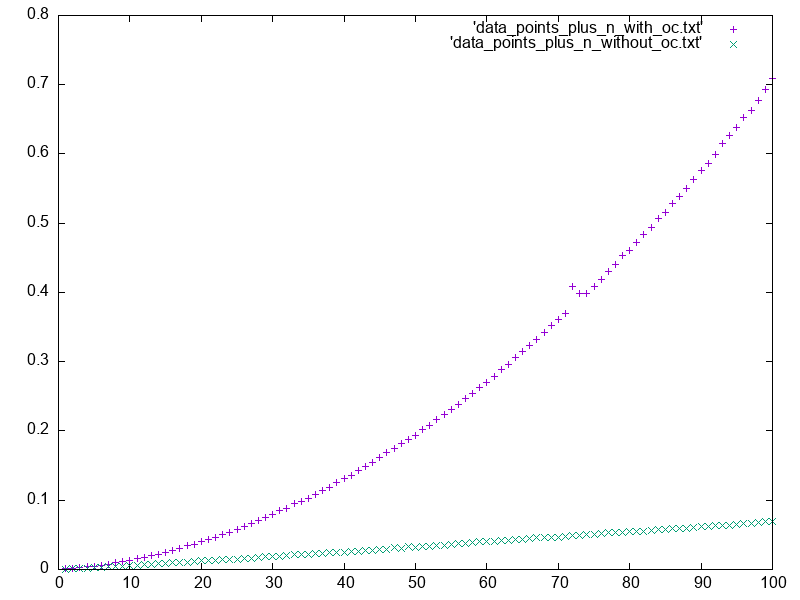
\includegraphics[width=10cm,height=8cm]{plot_example}
  \caption{The plot for the addition query showing dependency of total time (in seconds) of the search for the query \lstinline|length$^o$ $\,$ $\overline{n}$ $\,$ $\overline{m}$ $\,$ $\underline{l}$| of the value of $n$ with a fixed $m$. Purple dots show the time for the case when occurs checks are performed, green dots --- for the case when they are not performed. }
  \label{fig:plot_example}
\end{figure}

To check how well our estimates correspond to reality we implemented a simple embedding of \mK into OCaml and measured the time of the search for the example queries, building plots of time vs parameters in the estimated complexity (distinct plot for each parameter).~\footnote{The implementation and the results of the measuring can be found at \color{red}{\url{TODO}}} The referenced embedding follows the standard microKanren implementation but with standard library maps for substitutions and with possibility to switch occurs check on and off, for time measuring we are using standard OCaml "benchmark" library. The precision we were able to achieve is rather limited, so the plots are not always smooth and can have abnormalities (especially for small sizes of the input), but the dependency is usually clear. Because of the problems with precision, for now we are able to adequately measure only total time of the search, with or without occurs checks, so we are basically verifying only the \figureword~\ref{fig:examples_total_times}. 
The example of the resulting plot is shown in \figureword~\ref{fig:plot_example} (time of addition of two numbers depending on the first argument). The character of a time dependency function is not always visible from the plot (when the degree of the polynomial is greater than one), but after studying each plot individually (for example, by placing the plot between two polynomials of the same degree) we are reasonably sure that all complexity estimates from the \figureword~\ref{fig:examples_total_times} are accurate.
